%\documentclass[sigconf,authordraft]{acmart}
\documentclass[sigconf]{acmart}
\settopmatter{printacmref=false}
\renewcommand\footnotetextcopyrightpermission[1]{}

\AtBeginDocument{%
  \providecommand\BibTeX{{%
    \normalfont B\kern-0.5em{\scshape i\kern-0.25em b}\kern-0.8em\TeX}}}
    
\makeatletter
\DeclareRobustCommand{\textsupsub}[2]{{%
  \m@th\ensuremath{%
    ^{\mbox{\fontsize\sf@size\z@#1}}%
    _{\mbox{\fontsize\sf@size\z@#2}}%
  }%
}}
\makeatother

\usepackage[ruled,vlined,noend]{algorithm2e}
%\usepackage{algorithmic}
%\usepackage{algorithm}
\usepackage{mathtools}
\usepackage{amsthm}
\usepackage{cleveref}
\usepackage{setspace}
\usepackage{enumitem}
\usepackage{chngcntr}
%\usepackage[backend=biber]{biblatex}

\counterwithin{figure}{section}
\counterwithin{table}{section}

\newtheoremstyle{remboldstyle}
   {}{}{}{}{\bfseries}{.}{.5em}{{\thmname{#1 }}{\thmnumber{#2}}{\thmnote{ (#3)}}}
\theoremstyle{remboldstyle}
\newtheorem{theorem}{Theorem}[section]
\newtheorem{definition}[theorem]{Definition}
\newtheorem{corollary}[theorem]{Corollary}
\newtheorem{lemma}[theorem]{Lemma}
\newtheorem{remark}[theorem]{Remark}

\renewcommand{\theequation}{\arabic{section}.\arabic{equation}}
\counterwithin*{equation}{section}


\settopmatter{printfolios=true}

%%\usepackage[ruled,vlined]{algorithm2e}


\documentclass[sigconf]{acmart}
\settopmatter{printacmref=false} % Removes citation information below abstract
\renewcommand\footnotetextcopyrightpermission[1]{} % removes footnote with conference information in first column

\AtBeginDocument{%
  \providecommand\BibTeX{{%
    \normalfont B\kern-0.5em{\scshape i\kern-0.25em b}\kern-0.8em\TeX}}}
    
\makeatletter
\DeclareRobustCommand{\textsupsub}[2]{{%
  \m@th\ensuremath{%
    ^{\mbox{\fontsize\sf@size\z@#1}}%
    _{\mbox{\fontsize\sf@size\z@#2}}%
  }%
}}
\makeatother

\usepackage[ruled,linesnumbered,noend]{algorithm2e}
%\usepackage{algorithmic}
%\usepackage{algorithm}
\usepackage{mathtools}
\usepackage{amsthm}
\usepackage{cleveref}
\usepackage[vlined]{algorithm2e}
\newcommand{\vect2}[1]{\boldsymbol{#1}}
\newcommand{\Real}[0]{\mathbb{R}}
\newcommand{\Int}[0]{\mathbb{Z}}
\newcommand{\Nat}[0]{\mathbb{N}}
\usepackage{setspace}

\newtheoremstyle{remboldstyle}
   {}{}{}{}{\bfseries}{.}{.5em}{{\thmname{#1 }}{\thmnumber{#2}}{\thmnote{ (#3)}}}
\theoremstyle{remboldstyle}
\newtheorem{theorem}{Theorem}[section]
\newtheorem{definition}[theorem]{Definition}
\newtheorem{corollary}[theorem]{Corollary}
\newtheorem{lemma}[theorem]{Lemma}
\newtheorem{remark}[theorem]{Remark}

\renewcommand{\theequation}{\arabic{section}.\arabic{equation}}
\counterwithin*{equation}{section}

\usepackage{enumitem}
\newcommand{\dd}{\mathrm{d}}
\settopmatter{printfolios=true}

\makeatletter
\newcommand{\nosemic}{\renewcommand{\@endalgocfline}{\relax}}
\newcommand{\dosemic}{\renewcommand{\@endalgocfline}{\algocf@endline}}
\newcommand{\pushline}{\Indp}
\newcommand{\popline}{\Indm\dosemic}
\makeatother
\SetKwComment{Comment}{\vartriangleright\:\: }{}
\renewcommand{\nl}{}

%%\usepackage[ruled,vlined]{algorithm2e}


\documentclass[sigconf]{acmart}
\settopmatter{printacmref=false} % Removes citation information below abstract
\renewcommand\footnotetextcopyrightpermission[1]{} % removes footnote with conference information in first column

\AtBeginDocument{%
  \providecommand\BibTeX{{%
    \normalfont B\kern-0.5em{\scshape i\kern-0.25em b}\kern-0.8em\TeX}}}
    
\makeatletter
\DeclareRobustCommand{\textsupsub}[2]{{%
  \m@th\ensuremath{%
    ^{\mbox{\fontsize\sf@size\z@#1}}%
    _{\mbox{\fontsize\sf@size\z@#2}}%
  }%
}}
\makeatother

\usepackage[ruled,linesnumbered,noend]{algorithm2e}
%\usepackage{algorithmic}
%\usepackage{algorithm}
\usepackage{mathtools}
\usepackage{amsthm}
\usepackage{cleveref}
\usepackage[vlined]{algorithm2e}
\newcommand{\vect2}[1]{\boldsymbol{#1}}
\newcommand{\Real}[0]{\mathbb{R}}
\newcommand{\Int}[0]{\mathbb{Z}}
\newcommand{\Nat}[0]{\mathbb{N}}
\usepackage{setspace}

\newtheoremstyle{remboldstyle}
   {}{}{}{}{\bfseries}{.}{.5em}{{\thmname{#1 }}{\thmnumber{#2}}{\thmnote{ (#3)}}}
\theoremstyle{remboldstyle}
\newtheorem{theorem}{Theorem}[section]
\newtheorem{definition}[theorem]{Definition}
\newtheorem{corollary}[theorem]{Corollary}
\newtheorem{lemma}[theorem]{Lemma}
\newtheorem{remark}[theorem]{Remark}

\renewcommand{\theequation}{\arabic{section}.\arabic{equation}}
\counterwithin*{equation}{section}

\usepackage{enumitem}
\newcommand{\dd}{\mathrm{d}}
\settopmatter{printfolios=true}

\makeatletter
\newcommand{\nosemic}{\renewcommand{\@endalgocfline}{\relax}}
\newcommand{\dosemic}{\renewcommand{\@endalgocfline}{\algocf@endline}}
\newcommand{\pushline}{\Indp}
\newcommand{\popline}{\Indm\dosemic}
\makeatother
\SetKwComment{Comment}{\vartriangleright\:\: }{}
\renewcommand{\nl}{}

%%\usepackage[ruled,vlined]{algorithm2e}


\documentclass[sigconf]{acmart}
\settopmatter{printacmref=false} % Removes citation information below abstract
\renewcommand\footnotetextcopyrightpermission[1]{} % removes footnote with conference information in first column

\AtBeginDocument{%
  \providecommand\BibTeX{{%
    \normalfont B\kern-0.5em{\scshape i\kern-0.25em b}\kern-0.8em\TeX}}}
    
\makeatletter
\DeclareRobustCommand{\textsupsub}[2]{{%
  \m@th\ensuremath{%
    ^{\mbox{\fontsize\sf@size\z@#1}}%
    _{\mbox{\fontsize\sf@size\z@#2}}%
  }%
}}
\makeatother

\usepackage[ruled,linesnumbered,noend]{algorithm2e}
%\usepackage{algorithmic}
%\usepackage{algorithm}
\usepackage{mathtools}
\usepackage{amsthm}
\usepackage{cleveref}
\usepackage[vlined]{algorithm2e}
\newcommand{\vect2}[1]{\boldsymbol{#1}}
\newcommand{\Real}[0]{\mathbb{R}}
\newcommand{\Int}[0]{\mathbb{Z}}
\newcommand{\Nat}[0]{\mathbb{N}}
\usepackage{setspace}

\newtheoremstyle{remboldstyle}
   {}{}{}{}{\bfseries}{.}{.5em}{{\thmname{#1 }}{\thmnumber{#2}}{\thmnote{ (#3)}}}
\theoremstyle{remboldstyle}
\newtheorem{theorem}{Theorem}[section]
\newtheorem{definition}[theorem]{Definition}
\newtheorem{corollary}[theorem]{Corollary}
\newtheorem{lemma}[theorem]{Lemma}
\newtheorem{remark}[theorem]{Remark}

\renewcommand{\theequation}{\arabic{section}.\arabic{equation}}
\counterwithin*{equation}{section}

\usepackage{enumitem}
\newcommand{\dd}{\mathrm{d}}
\settopmatter{printfolios=true}

\makeatletter
\newcommand{\nosemic}{\renewcommand{\@endalgocfline}{\relax}}
\newcommand{\dosemic}{\renewcommand{\@endalgocfline}{\algocf@endline}}
\newcommand{\pushline}{\Indp}
\newcommand{\popline}{\Indm\dosemic}
\makeatother
\SetKwComment{Comment}{\vartriangleright\:\: }{}
\renewcommand{\nl}{}

%\input{common}

\begin{document}


\begin{document}


\begin{document}


\begin{document}

\newcommand{\dd}{\mathrm{d}}
\newcommand{\vect}[1]{\boldsymbol{#1}}
\newcommand{\Real}[0]{\mathbb{R}}
\newcommand{\Int}[0]{\mathbb{Z}}
\newcommand{\Nat}[0]{\mathbb{N}}

\makeatletter
\newcommand{\nosemic}{\renewcommand{\@endalgocfline}{\relax}}
\newcommand{\dosemic}{\renewcommand{\@endalgocfline}{\algocf@endline}}
\newcommand{\pushline}{\Indp}
\newcommand{\popline}{\Indm\dosemic}
\makeatother
\SetKwComment{Comment}{\vartriangleright\:\: }{}
%\renewcommand{\nl}{}

%%
%% The "title" command has an optional parameter,
%% allowing the author to define a "short title" to be used in page headers.
\title{The Numerical Analyses of Global Optimization and Simulated Annealing}
%\subtitle{A Comprehensive Summary and Analysis of Dekkers' and Aarts' "Global Optimization and Simulated Annealing"}

%%
%% The "author" command and its associated commands are used to define
%% the authors and their affiliations.
%% Of note is the shared affiliation of the first two authors, and the
%% "authornote" and "authornotemark" commands
%% used to denote shared contribution to the research.
\author{Jacques Nel}
\authornote{All authors contributed equally to this research.}
\email{jmn23@my.yorku.ca}
\affiliation{%
  \institution{}
  %\streetaddress{P.O. Box 1212}
  \city{ID. 212588109}
  \state{}
  \postcode{43017-6221}
}

\author{Celina Landolfi}
\authornotemark[1]
\email{clandolfi17@gmail.com}
\affiliation{%
  \institution{}
  %\streetaddress{P.O. Box 1212}
  \city{ID. 215587892 }
  \state{}
  \postcode{43017-6221}
}

\author{Gian Alix}
\authornotemark[1]
\email{gian.alix@gmail.com}
\affiliation{%
  \institution{}
  %\streetaddress{P.O. Box 1212}
  \city{ID. 214760870}
  \state{}
  \postcode{43017-6221}
}


%%
%% By default, the full list of authors will be used in the page
%% headers. Often, this list is too long, and will overlap
%% other information printed in the page headers. This command allows
%% the author to define a more concise list
%% of authors' names for this purpose.

%%
%% The abstract is a short summary of the work to be presented in the
%% article.
% \begin{abstract}
%   This assignment is about three network models and their properties: 
%   Erdős-Rényi random graph model, Watts–Strogatz small-world graph model and Barabási–Albert preferential attachment model.
% \end{abstract}

%%
%% The code below is generated by the tool at http://dl.acm.org/ccs.cfm.
%% Please copy and paste the code instead of the example below.
%%
% \begin{CCSXML}
% <ccs2012>
%  <concept>
%   <concept_id>10010520.10010553.10010562</concept_id>
%   <concept_desc>Computer systems organization~Embedded systems</concept_desc>
%   <concept_significance>500</concept_significance>
%  </concept>
%  <concept>
%   <concept_id>10010520.10010575.10010755</concept_id>
%   <concept_desc>Computer systems organization~Redundancy</concept_desc>
%   <concept_significance>300</concept_significance>
%  </concept>
%  <concept>
%   <concept_id>10010520.10010553.10010554</concept_id>
%   <concept_desc>Computer systems organization~Robotics</concept_desc>
%   <concept_significance>100</concept_significance>
%  </concept>
%  <concept>
%   <concept_id>10003033.10003083.10003095</concept_id>
%   <concept_desc>Networks~Network reliability</concept_desc>
%   <concept_significance>100</concept_significance>
%  </concept>
% </ccs2012>
% \end{CCSXML}

% \ccsdesc[500]{Computer systems organization~Embedded systems}
% \ccsdesc[300]{Computer systems organization~Redundancy}
% \ccsdesc{Computer systems organization~Robotics}
% \ccsdesc[100]{Networks~Network reliability}

%%
%% Keywords. The author(s) should pick words that accurately describe
%% the work being presented. Separate the keywords with commas.
\keywords{global optimization, simulated annealing, continuous variables}



%%
%% This command processes the author and affiliation and title
%% information and builds the first part of the formatted document.
\maketitle

\section{Introduction}
\label{sec:intro}

Global optimization, a branch of applied mathematics and numerical analysis, is concerned with finding points on a bounded subset $S$ of $\mathbb{R}^n$ in which some function $f$ assumes its optimal value \cite{dekkers}. The function may have numerous local optima values and instead of searching for local points that cannot be improved, global optimization aims to find the global optimum on the bounded subset \cite{neumaier}. Thus, global optimization is a stronger version of local optimization and is desirable, but not necessary, in many practical applications; however, there are several applications where the use of global optimization is crucial including problems in safety verification, chemistry and hard feasibility problems \cite{neumaier}. In these cases, using local optimization methods could potentially return useless information, could be unrealistic with respect to the real world or could potentially underestimate the problem at hand \cite{neumaier}. Despite the obvious importance of global optimization and the efforts that have been invested into developing algorithms, the results have been unsatisfactory thus far and more work is needed for the optimization of more complicated functions \cite{dekkers}. Currently, numerical methods are used for the optimization of complicated functions, but these often cannot produce optimal results and will return a value close to a global optimum instead. By 'close to', we mean the following:

\begin{definition}['Close To' Global Minimum]
For $\epsilon > 0, B_f(\epsilon) $ is the set of points with a value close to the minimal point, i.e.
\begin{equation}
    B_f(\epsilon)=\{x \in S |\exists_{{x}_{min}}:|f(x)-f({x}_{min})|<\epsilon \}
\end{equation}
\end{definition}

Furthermore, we construct a formal definition for what it means for a set of points to be close to a minimal point:
\begin{definition}
Let $\epsilon$ be any positive real number. Then we define $B_x(\epsilon)$ to be the set such that:
\begin{equation}
    B_x(\epsilon) = \{ x \in S \, | \, \exists x_{\min} \, : \, ||x-x_{\min}|| < \epsilon \}
\end{equation}
and this is a set containing all points close to the minimal.
\label{def:close-to-min}
\end{definition}

There are two classes of numerical methods in regards to global optimization: deterministic, in which the minimization process depends on probabilistic events, and stochastic methods, which does not use probabilistic information \cite{dekkers}. Unfortunately, deterministic global optimization methods have several disadvantages including that the global optimum can only be found after an exhaustive search over $S$, there is no guarantee of success from the method and that many assumptions must be made about $f$ \cite{dekkers}. On the other hand, stochastic methods generally have better computational results than deterministic methods and can almost all be proven to find a global optimum that is asymptotically convergent with probability 1 \cite{dekkers}. With this taken into consideration, the concentration of global optimization methods will be on stochastic methods, specifically simulated annealing. 




\section{Problem Definition}
\label{sec:prob}

Let $S\subset\mathbb{R}^n$ be a bounded set on $\mathbb{R}^n$ and $f:S\to\mathbb{R}^n$ be an $n$-dimensional real-valued function. \\
The problem that simulated annealing wishes to solve is to find a point $x_{min} \in S$ such that $f(x_{min})$ is a global minimum on $S$. \\
\\
Specifically, 
\begin{equation}
    \forall x \in S : f(x_{\min}) \leq f(x)
    \label{eq:min-def}
\end{equation}

The problem deals with global minimization; however, simulated annealing can find global maximization in the same way by reversing the sign of $f$ without loss of generality [1].

\section{The Numerical Method}
\label{sec:related}

Since local optimality does not guarantee global optimality, a fundamental concern in global optimization is getting stuck at a local optimum point \cite{dekkers}. In order to avoid and overcome this, a specific class of stochastic optimization is used, which is simulated annealing. Simulated annealing originates from the physical annealing process that is well known in condensed matter physics \cite{dekkers}. Physical annealing is a thermal process where the heating and slow cooling of a metal in a heat bath brings it into a more uniformly crystalline state where the free energy takes its global minimum. The role of temperature in physical annealing is to allow the particles to reach higher energy states in order to overcome energy barriers that would force them into local minima \cite{neumaier}. \\
\hspace*{3mm}In greater detail, a state with energy level $E_1$ is compared to a state with energy level $E_2$, which is obtained by moving one of the particles into another location by a small displacement. $E_2$ is only accepted if the movement of the particle brings the system in a state of lower energy (i.e. $E_2-E_1\leq0$). If this is not the case, a movement to a state of higher energy $E_2$ (also called a deterioration) is only accepted with probability 
$e^-{\frac{(E_2-E_1)}{kT}}$, where $k$ is the Boltzmann constant and $T$ is the temperature \cite{dekkers}. However, the probability of accepting these deteriorations descends slowly towards zero as this process continues. Thus, the repetition of this process for a large enough number of particle movements using this stochastic acceptance criterion for deteriorations make it possible to overcome becoming stuck at local minima and leads to a (near) global minima \cite{dekkers}.\\
\hspace*{3mm}In 1983, Kirkpatrick, Gellatt and Vecchi applied the physical annealing of metal with combinatorial minimization by replacing energy with a cost function and the movement of the particles in the physical system became analogous to a trial in the combinatorial minimization problem \cite{dekkers}. This algorithm proves to have many benefits when applied to combinatorial minimization problems including guarantee of convergence to global minimum, generally applicable to the cost function and easy to implement with good performance \cite{dekkers}. \\
\hspace*{3mm}The approach of the simulated annealing algorithm is to generate homogeneous Markov chains of finite length at a finite sequence of descending values of the control parameter \cite{dekkers}. The cooling schedule consists of a set of parameters that controls the convergence of the algorithm, as listed below: \\
\begin{itemize}
\item initial value of the control parameter $c$ 
\item a decrement function for decreasing the value of the control parameter $c$
\item a stop criterion
\item a finite length, $L$, of each Markov chain\\ \cite{dekkers}   
\end{itemize}

The parameters of the cooling schedule are described below in more detail.

\subsection{Initial value of the control parameter ($c_0$)}

The basic assumption regarding the initial value of the control parameter is that $c_0$ should be sufficiently large such that approximately all transitions are accepted at this value. If we let $\chi(c)$ denote the ratio between the number of accepted transitions and number of accepted transitions along the Markov chain at $c$. The problem of determining $c_0$ can be posed in terms of requiring
the initial acceptance ratio $\chi_0=\chi(c_0)$ to be close to 1.

The authors of \cite{dekkers} propose that $c_0$ be determined by the following scheme: The objective function $f(\vect{x})$ is sampled
$m$ times with $\vect{x} \sim \mathrm{Uniform}\left( \mathcal{S}\right)$. Let $\Delta f = f(\vect{y}) - f(\vect{x})$, and
$\Delta f^+ = \left\lbrace \Delta f : \Delta f > 0 \right\rbrace$. Let $m_1$ denote the number of accepted transitions, with
$m=m_1+m_2$, and let $\overline{\Delta f^+}$ be the average values of $\Delta f_{xy}$ for which $\Delta f_{xy}>0$

\begin{equation}
\label{eq:3-2}
    c_0 = \overline{\Delta {f}^+} \, \Bigg(\ln \dfrac{m_2}{m_2 \chi_0+(1-\chi_0)m_1} \Bigg)^{-1} 
\end{equation}

In practice, \cref{eq:3-2} was found to be problematic. The logarithm can result in a negative $c_0$ which does not make sense.
Furthermore, if $m$ is not sufficiently large, $c_0$ exhibits very high variance. This occurs because the mean in 
$\overline{\Delta f^+}$ is very sensitive to extreme values. Quick examination of the histograms of $\Delta f^+$ of the Rosenbrock
test function suggested that $\Delta f^+$ is heavy-tailed.

Instead let's suppose we want the $\chi_0$-th quantile transition to have a high ($p=0.9)$ probability of being accepted. 
\Cref{fig:acceptance} shows that $\exp -\Delta f / c$ maps $\Delta f$ onto a probability. If we let $k=\chi$-th quantile of the
$\Delta f^+$ values, we can determine $c_0$ with


\begin{equation}
    \label{eq:schedule_init}
    \exp - \frac{k}{c_0} \geq p \implies c_0 = -\frac{k}{\log p}
\end{equation}

\begin{figure}
    \centering
    \textbf{Affect of $c$ on acceptance probability}
    %\caption{}
    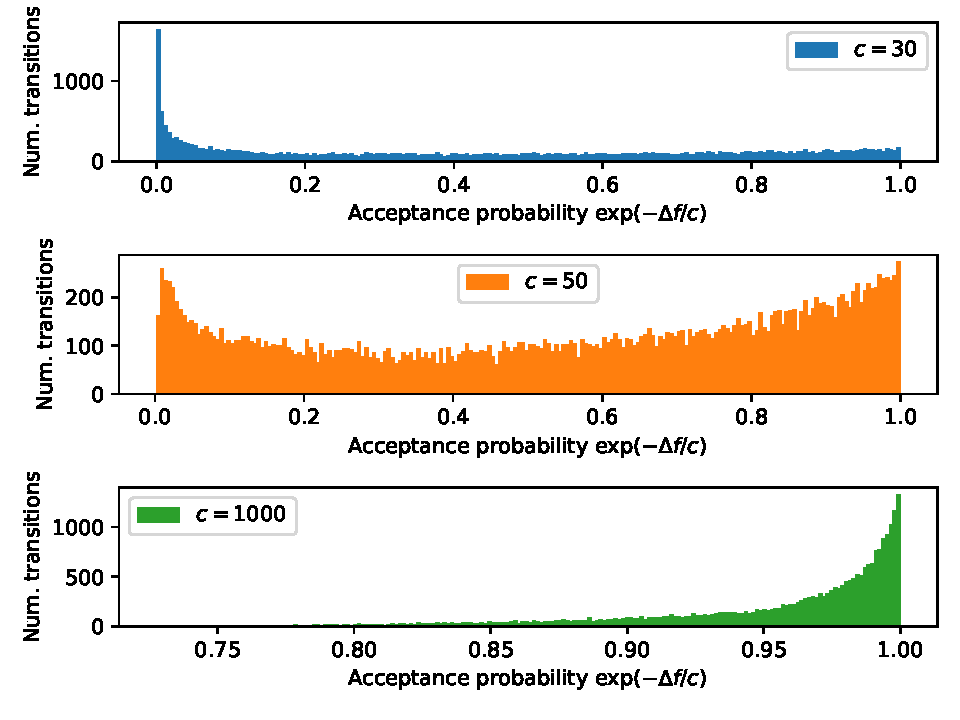
\includegraphics[scale=0.5]{figures/fig33.pdf}
    \label{fig:acceptance}
    
  \caption{Using the Rosenbrock function, 50,000 transitions were computed. Among those, the positive transitions were selected and the exponential function $exp(-\Delta f/c)$  was applied and used as the acceptance criterion. Using three different $c$ values of 30, 50 and 1000, it is shown that a greater value of $c$ leads to more transitions given a higher probability of being accepted.}
\end{figure}

\subsection{Decrement of the control parameter}
The decrement function is used to decrease the value of $c$\\
The new value of $c$, $c'$ is calculated by:
\begin{equation}\label{eq:c_dec}
    c'=c \, \Bigg(1+\dfrac{c\ln(1+\delta)}{3\sigma (c)}\Bigg)^{-1} 
\end{equation} 
where $\sigma(c)$ is the standard deviation of the values of the cost function of the points of the Markov chain at $c$ and the constant $\delta$ is the distance parameter that determines the speed of the decrement of the control parameter $c$ \cite{dekkers}.

Particular care must be given towards the $\sigma(c)$ term in the denominator of \cref{eq:c_dec}. Especially when $c$ is small, towards
the later stages of the annealing schedule, a Markov chain at the current $c$ can fail to make any transitions. In such situations,
$\sigma(c) = 0$, and we have both a divide-by-zero exception, and $c$ can be set to 0 prematurely, which has the result of triggering
the stop condition, before a good solution is reached.

One way to address this issue is to repeatedly sample a Markov chain until some minimum number of transitions are performed. Due to
descent direction component of point generation alternative B, the Markov chain will usually make at least one transition, even
if it is very small, thus avoiding the divide-by-zero problem.

\begin{figure}[h]
    \centering
    \caption{Cooling schedule for Branin}
    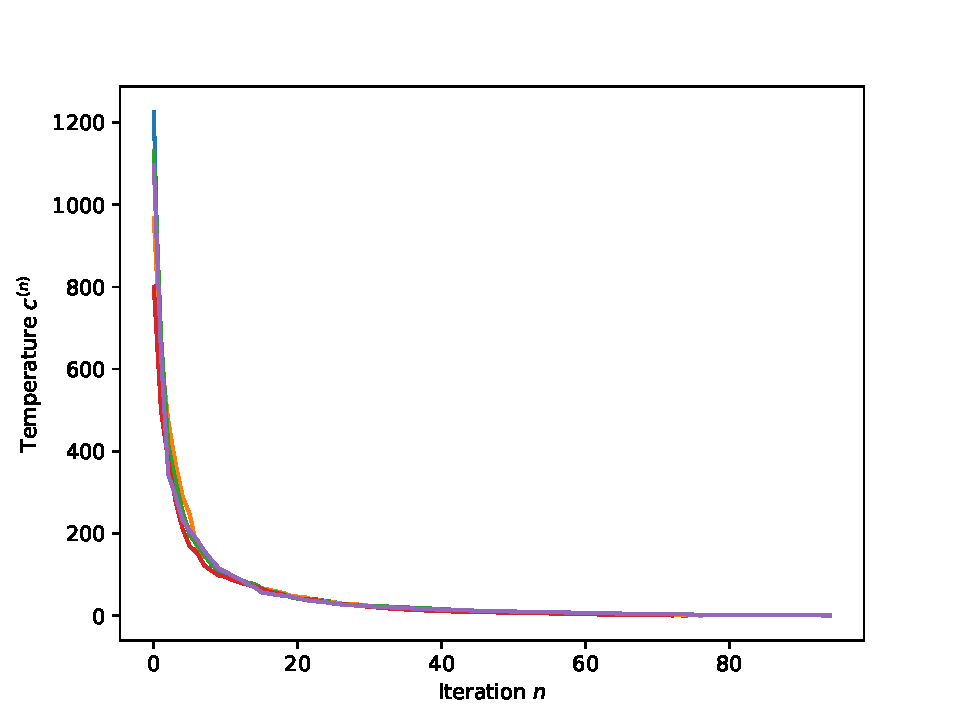
\includegraphics[scale=0.42]{figures/fig31-branin.pdf}
    \label{fig:512}
\end{figure}

\begin{figure}[h]
    \centering
    \caption{Cooling schedule for Goldstein-Price}
    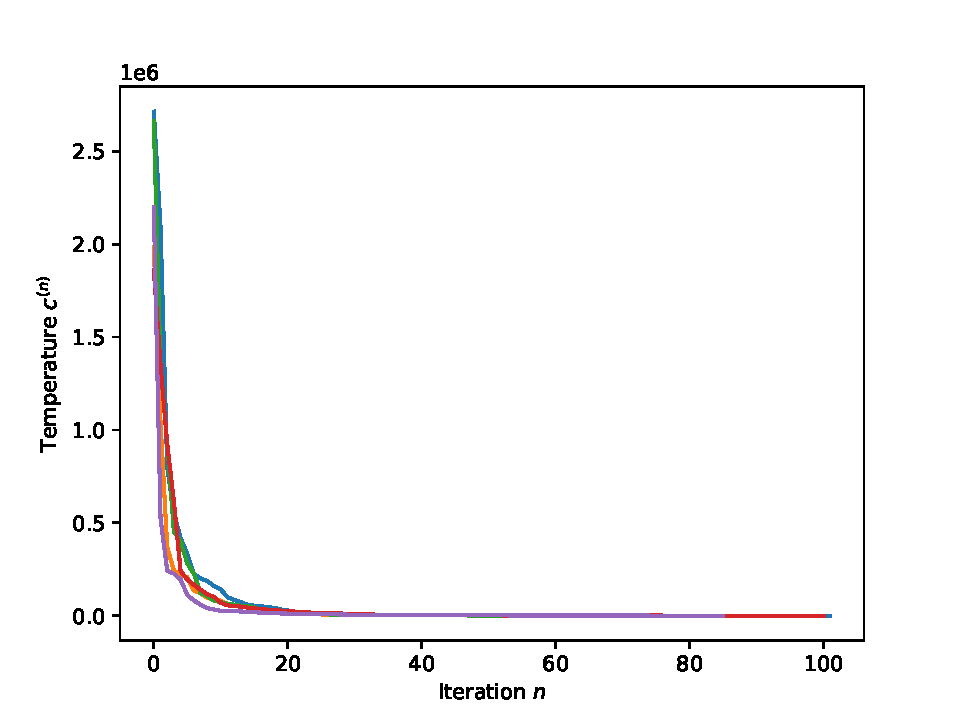
\includegraphics[scale=0.42]{figures/fig31-goldstein_price.pdf}
    \label{fig:512}
    \caption*{Figure 2 and Figure 3 represent an example Cooling Schedule for Branin and Golden-Price respectively, where each colour on the curve represents a different run, for 4 total runs.}
\end{figure}

\subsection{Stop condition}

Particular care needs to be given to devising an appropriate stopping condition.
First, let $\overline{f}(c_0)$ denote the mean value of the points in the initial Markov chain, and $\overline{f}(c)$ denote
the average values of the points in the chain at $c$. Then $\overline{f_s}(c)$ is the smoothed value of $\overline{f}$
over a number of chains in order to reduce fluctuations of $\overline{f}(c)$. In practice the smoothing is applied
using a small smoothing parameter $0 < \gamma < 1$ and

\begin{equation}
    \label{smoothing}
    \begin{array}{c}
    \overline{f_s}^{(n+1)} = \gamma \overline{f}^{(n+1)} + (1-\gamma) \overline{f_s}^{(n)} \\
    \\
    \overline{f_s}^{(0)} = \overline{f}^{(0)} \\
    \end{array}
\end{equation}

The algorithm is terminated if:
\begin{equation}
\label{eq:stop_cond}
    \Bigg|\frac{d \overline{f_s}(c)}{dc} \frac{c}{\overline{f}(c_0)} \Bigg| < \epsilon_s 
\end{equation}

where $\epsilon_s$ is the stop parameter, a small positive real number. The derivative in \cref{eq:stop_cond}
is simply calculated using a finite difference method \cite{dekkers}.
 
%\begin{itemize}
%\item$\overline{f}(c_0)$ is the mean value of the points found in the initial Markov chain
%\item $\overline{f_s}(c)$ is the smoothed value of $\overline{f}$ over a number of chains in order to reduce %fluctuations of $\overline{f}(c)$ and
%\item $\epsilon_s$ is the stop parameter, a small positive real number.
%\end{itemize}

\subsection{Length of the Markov chains}
Let $n$ be the dimension of $S$ and let $L_0$ be a constant called the standard length. Then 
\begin{equation}
    L=L_0 \cdot n     
\end{equation}
is the length of the Markov chain, which must be sufficiently large in order to enable the algorithm to explore the neighbourhood of a given point in all directions \cite{dekkers}. \vspace{5pt}

A pseudo-code for the algorithm can be found in \textbf{Algorithm \ref{algo:sa}}.


\begin{algorithm}
\setstretch{1.4}
\caption{Simulated Annealing}\label{algo:sa}
\vspace{8pt}
\nosemic
\SetAlgoLined
\KwIn{
$f:\mathcal{S} \longrightarrow \Real, 
\nabla f, 
\mathcal{S}, 
l_0,
\epsilon_s,
\gamma$
}

$l \longleftarrow l_0 \cdot \texttt{dim}(\mathcal{S}) $ \;
$c_0 \longleftarrow \texttt{init\_schedule}(\mathcal{S}, \chi, m) $ \;

$c  \longleftarrow c_0$ \;

$\vect{x} \longleftarrow \texttt{gen\_point\_a}(\mathcal{S})$ \;

f\_x $\longleftarrow f(\vect{x})$ \;

\While{true}
{
    f\_at\_c \longleftarrow $\left\lbrace f(\vect{x}) \right\rbrace$ \;

    chain $\longleftarrow \left\lbrace \: \right\rbrace$ \;

    \For{ $i \in \left\lbrace 1, \ldots, l\right\rbrace$} {

        $\vect{y} \longleftarrow \texttt{gen\_point\_b}(\vect{x}, f, \nabla f,\mathcal{S}, t )  $ \;

        f\_y $\longleftarrow f(\vect{y})$ \;

        $\Delta \longleftarrow $ f\_y - f\_x \;

        \Comment{a}
        \If{ $\Delta \leq 0$ or $\exp\left( -\Delta /c ) > \texttt{random}[0,1) $ }
        {
            $\vect{x} \longleftarrow \vect{y} $ \;

            chain$.\texttt{push}(\vect{y})$ \;
            f\_at\_c$.\texttt{push}($ f\_y $)$\;

            f\_x $\longleftarrow$ f\_y \;


        }


    }

    $\overline{f} \longleftarrow \texttt{mean}(f\_at\_c)$ \;
    $\sigma \longleftarrow \texttt{std}(f\_at\_c)$ \;

    \If{ $\sigma = 0$ }{
        $\sigma \longleftarrow 10^{-14}$ \;
    }

    \uIf{ $n= 0$ } {
        $\overline{f}_s \longleftarrow \overline{f}$ \;
        $\overline{f}_0 \longleftarrow \overline{f}$ \;

    } 
    \uElse {
    $\overline{f}_s^{(0)} \longleftarrow \overline{f} $ \;

    $\overline{f}_s = (1 - \gamma) \overline{f}_s + \gamma \overline{f} $\;
}

    $c_{n-1} \longleftarrow = c$ \;

    $
    c \longleftarrow c\left(1 + \log\frac{1 + \delta}{3 \sigma}\right)^{-1}
    $

    dc $\longleftarrow c - c_{n-1}$ \;

    \If{ $n > 0$ and dc $ \neq 0$ } {
        $d\overline{f}_s \longleftarrow \overline{f}_s - \overline{f}_s^{(0)}$ \;

        \vspace{5pt}

        \If{
        $\displaystyle\left| \frac{d\overline{f}_s }{dc}\frac{c}{\overline{f}_0} \right| < \epsilon_s $ }
        {
            \Return{$\vect{x}^\star = \vect{x}, f(\vect{x}^\star)$ } \;
        }
        
        \vspace{5pt}
    }

    $n \longleftarrow n+1 $ \;

}

\end{algorithm}

\begin{algorithm}
\setstretch{1.4}
\caption{Init. schedule - \texttt{init\_schedule}}\label{algo:sa}
\vspace{8pt}
\nosemic
\SetAlgoLined

\KwIn{
$f:\mathcal{S} \longrightarrow \Real, 
\mathcal{S}, 
\chi,
m$
}

$\vect{x}_0 \longleftarrow$ gen\_point\_a( $\mathcal{S}$ ) \;

\For{i $\in \left\lbrace 1, \ldots m-1\right\rbrace$} {
    $\vect{x}_i \longleftarrow $ gen\_point\_b( $\vect{x}_{i-1}$ ) \;
}

$\Delta_i = f(\vect{x}_{i+1}) - f(\vect{x}_i)$ for $i = 0,\ldots m-1$ \;

$\Delta^+ = \left\lbrace \Delta_i : \Delta_i > 0 \right\rbrace $ \;

cutoff $\longleftarrow$ $\chi$-quantile( $\Delta^+$ ) \;

$C_0 \longleftarrow -\text{ cutoff} / \log(\chi)$ \;

\Return{$C_0$} \;


\end{algorithm}

\begin{algorithm}
\setstretch{1.4}
\caption{Generate point alternative A - \texttt{gen\_point\_a}}\label{algo:sa}
\vspace{8pt}
\nosemic
\SetAlgoLined
\KwIn{
    $\mathcal{S}$
}

$\vect{x} \longleftarrow$ sample(Uniform($\mathcal{S})) $ \;

\Return{$\vect{x}$}

\end{algorithm}

\begin{algorithm}
\setstretch{1.4}
\caption{Generate point alternative B - \texttt{gen\_point\_b}}\label{algo:gen-b}
\vspace{8pt}
\nosemic
\SetAlgoLined
\KwIn{
$f:\mathcal{S} \longrightarrow \Real, 
\nabla f, 
\mathcal{S}, t$
}

$w \longleftarrow $ random( $[0,1)$ ) \;

\If{$w > t$}
{
    $\vect{x} \longleftarrow $ sample( Uniform( $\mathcal{S}$ ) ) \;
} \uElse {
    
    $\vect{x} \longleftarrow \texttt{grad\_descent}(f, \nabla f, \vect{x_0}, N=1 )$ \;
}

\Return{$\vect{x}$}

\end{algorithm}

%$f^\star \longleftarrow \infty$\;

%\;

%\For{$n\in \left\lbrace 1,\ldots, N\right\rbrace$}{
%$\vect{x}_0 \longleftarrow \mathrm{Uniform}\left(\mathcal{S}\right)$ \Comment*{random sample init. point}

%$x_l = \texttt{steepest\_descent}(f, \nabla f, \vect{x}_0, \tau)$ \;

%\If{$f(\vect{x}_l) \leq f^\star$}{
%    $f^\star \longleftarrow f(\vect{x}_l)$ \;
%    
%    $\vect{x}^\star \longleftarrow \vect{x}_l$ \;
%}

%\uIf{$n=0$}{
%    $f^\star_s \longleftarrow C$ \Comment*{$0< C \in\Real$ to prevent 0}
%    $f^\star_s^{(0)} \longleftarrow f_s^\star$ \;
%} \uElse{
%    $f^\star_s^{(0)} \longleftarrow f^\star_s$ \;
%    $f^\star_s = \gamma f^\star + (1-\gamma)f^\star_s^{(0)}$
%    \;
%    \Comment{Stop when smoothed improvement reaches 0}
%    $\Delta_s = f^\star_s^{(0)} - f^\star_s$ \;
%    
%    \Comment{Check stop condition}
%    \If{ $\Delta_s \leq \epsilon_s$}{
%        \KwOut{Solution found $\vect{x}^\star$}
%    }
%}

%\;
%\KwOut{Failed to find solution in $N$ iterations, $\vect{x}^\star$}\;
%}
%\end{algorithm}

%\begin{algorithm}[t]
%\caption{\textsc{Simulated Annealing}}
%\begin{algorithmic}
%\STATE begin
%\STATE "initialize $(c,x)$;"
%\STATE stopcriterion := false;
%\WHILE{stopcriterion = false} 
%\STATE begin
%\FOR{$i$:=1 \TO $L$}
%\STATE begin
%\STATE "generate $y$ from $x$";
%\IF{$f(y)-f(x) \leq 0$}
%\STATE accept
%\ELSIF{$\exp{(-(f(y)-f(x))/c)} > \textsc{random}[0,1)$}
%\STATE accept;
%\IF{accept}
%\STATE $x:=y$
%\ENDIF
%\ENDIF
%\STATE "lower c"
%\ENDFOR
%\ENDWHILE
%\end{algorithmic}
%\label{algo:sa}
%\end{algorithm}

\subsection{Generation of Points} 
\label{sec:gen-points}
There are several ways to generate new points from a given point and two alternatives are used for the purposes of this project, Alternative A and Alternative B:
\begin{enumerate}[label=\textbf{(\Alph*)}]
    \item A uniform distributions on $S$:
    \begin{equation}
        g_{xy}=\frac{1}{m(S)} 
    \end{equation}
A disadvantage about Alternative A is that no structural information about function values is used \cite{dekkers}.
    \item Either a point is drawn from a uniform distribution over $S$ or a step is made into a descent direction from the current point:
    \begin{equation}
    g_{xy}=\begin{cases}
          LS(x) \quad &\text{if} \, w>t \\
          \dfrac{1}{m(S)} \quad &\text{if} \, w \leq t \\
     \end{cases} 
    \end{equation}
    where $t$ is a fixed number in the interval [0,1) and $w$ is a random number from $U$[0,1). LS(x) is a Local Search procedure (i.e Steepest Descent Method) that generates a point $y$ in a descent direction of $x$. \cite{dekkers}

\end{enumerate}




 

\section{Theoretical Results}
\label{sec: methodology}
The mathematical model of the simulated annealing algorithm is based on the theory of Markov chains and thus, the following definitions are necessary: \vspace{5pt}

\begin{definition}[Markov Chains]
A \textit{Markov chain} in the simulated annealing algorithm is a sequence of trials. $X(k)$ is a random variable denoting the $k$th trial by simulated annealing, and the outcome of a trial is a point $x \in S$ that is dependent on the previous trial.
\end{definition}

\begin{definition}[The Generation Probability Distribution]
$g_{xy}$, as seen in \textbf{Section \ref{sec:gen-points}}, is the \textit{generation probability distribution}. That is, $g_{xy}$ is the probability distribution function for generating a point $y$ from point $x$ at a fixed value of the control parameter $c$.
\end{definition}

\begin{definition}[Acceptance Probability]
$A_{xy}$ is the \textit{acceptance probability}. That is, $A_{xy}$ is the probability of accepting point $y$ as a possible new point if $x$ is the current point in a Markov chain.
\end{definition}

\begin{definition}[Transition Probability]
A point $x \in S$ transformed to a point $y \in T \subset S$,  with the probability of generating and accepting a point in $T$ given that $x \notin T$ is called a \textit{transition probability}. Hence, for any current point $x$ in the Markov Chain, then the probability that an element in $T$ is the next point of the chain is given as:
\begin{equation}
    P(T \, | \, x; \, c) = \begin{dcases}
        \hfil \int_{y \in T} p_{xy}(c) \, \dd y & \text{for } x \notin T \\
        \int_{y \in T} p_{xy}(c) \, \dd y + \Bigg( 1 - \int_{y \in S} p_{xy}(c) \, \dd y \Bigg) & \text{for } x \in T \\
    \end{dcases}
\end{equation}
where
\begin{equation}
    p_{xy}(c) = g_{xy} \cdot A_{xy}(c)
\end{equation}
and
\begin{equation}
    P(T \, | \, x; \, c) = \mathbb{P}\{ X(l) \in T \, | \, X(l-1) = x\, ;\, c \}
\end{equation}
\end{definition}

\subsection{Asymptotic Convergence of the Algorithm}

Before asymptotic convergence of the algorithm is proved, the following definitions are necessary:

\begin{definition}[Stationary Probability Distribution Function]
A probability distribution function $r(x,c)$ is said to be \textit{stationary} if the following two conditions are met:
\begin{align}
    (1)\, & \, \forall_{x \in S}:r(x,c)=\int_{y \in S} r(y,c)p_{yx}(c) \dd y &  \notag \\
    & \hspace{25mm} + r(x,c) \Bigg( 1-\int_{y \in S} p_{xy}(c) \, \dd y \Bigg) &  \\
    (2) \,& \, \int_{x \in S} r(x,c) \dd x =1
\end{align}
\end{definition}

From this definition, the following is a stationary probability distribution since it meets the two conditions, which will later be used to show that the simulated annealing algorithm converges to a near minimal solution:
\begin{equation}
    q(x,c)=\exp{\Bigg( -\dfrac{f(x)-f_{\min}}{c} \Bigg)} \Bigg[ \int_{y \in S} \exp{\Bigg( -\dfrac{f(y)-f_{\min}}{c} \Bigg)}  \dd y \Bigg]^{-1}
    \label{eq:qxc}
\end{equation}


\begin{definition}[Probability of Transformation]
The probability that a point $x \in S$ is transformed into a point $y \in T \subset S$ in $k$ trials is:\\
\begin{equation}
    P^{(k)}(T \, | \, x; \, c) = \begin{dcases}
        \hfil \int_{y \in T} p^{(k)}_{xy}(c) \, \dd y & \text{for } x \notin T \\
        \int_{y \in T} p^{(k)}_{xy}(c) \, \dd y + \Bigg( 1 - \int_{y \in S} p_{xy}(c) \, \dd y \Bigg)^{k} & \text{for } x \in T \\
    \end{dcases}
\end{equation}
where
\begin{align}
    p^{(k)}_{xy}(c) &=\int_{z \in S} p^{(k-1)}_{xz}(c)p_{zy}(c) \, \dd z & \notag \\
    & \hspace{10mm} +p^{(k-1)}_{xz}(c) + \Bigg( 1 - \int_{z \in S} p_{yz}(c) \, \dd z \Bigg) & \notag \\
    & \hspace{10mm} + \Bigg( 1 - \int_{z \in S} p_{xz}(c) \, \dd z \Bigg)^{k-1}p_{xy}(c) 
\end{align}
i.e. $p^{(k)}_{xy}(c)$ is the quasi probability distribution function of transforming $x$ into $y$ in $k$ trials. $p^{(k)}_{xy}(c)$ is the summation of three terms, which are outlined below:\\
(i). Term 1: the quasi probability distribution function of transforming $x$ into $z$ in $k-1$ trials, and from $z$ to $y$ in the next trial integrated over all $z$. \\
(ii). Term 2: the quasi probability distribution function of transforming $x$ into $y$ in $k-1$ trials and then rejecting the $k$th trial. \\
(iii). Term 3: the quasi probability distribution function of transforming $x$ into $y$ in one trial after $k-1$ rejected trials from $x$.









\end{definition}


% Celina to insert Def2.5, 2.6 and Eq.2.36 above this line
% =============
In \textbf{Eq. (\ref{eq:qxc})}, we present a stationary probability distribution function, which is the necessary requirement for the Simulated Annealing algorithm to converge to the minimum solution. We present the theorem that:
\begin{theorem}
If there is a finite number of local minima for a uniformly continuous function $f$, then:
\begin{equation}
    \forall \epsilon > 0 \, : \, \lim_{c \rightarrow 0} \int_{y \in B_f(\epsilon)} q(y,c) \, \dd y > 1-\epsilon
\end{equation}
\label{thm:convergence-sa}
\begin{proof}
For a finite number of local minima, we have:
\begin{eqnarray}
    && \exists \epsilon_1 > 0 \, : \, |f(x_{\text{loc}}) - f_{\min}| > \epsilon_1 \\
    && \exists \epsilon_2 > 0, \, \forall x_{\min} \, : \, ||x_{\text{loc}} - x_{\min}|| > \epsilon_2 
    \label{eqn:x-loc-x-min}
\end{eqnarray}
where $f_{\min} = f(x_{\min})$, $\forall x_{\min}$ as per \textbf{Eq. (\ref{eq:min-def})} and $x_{\text{loc}}$ is a local, non-global minimum point. Then pick a positive $\epsilon$ such that: 
\begin{equation}
    \epsilon < \dfrac{1}{4}\min \{ \epsilon_1, \epsilon_2 \}
    \label{eqn:eps-one-fourth-min}
\end{equation}
It should be noted that if all minima are global, then select $\epsilon$ such that $\exists x \in S : f(x) - f_{\min} > \epsilon$. \vspace{5pt}

\noindent As $f$ is uniformly continuous, then:
\begin{equation}
    \exists \delta_1 > 0, \, \forall x,y \in S : ||x-y|| \leq \delta_1 \Longrightarrow |f(x)-f(y)| < \dfrac{\epsilon}{2}
\end{equation}
Choosing a $\delta$ such that $\delta = \min \{ \delta_1/2, \epsilon \}$, we have:
\begin{equation}
    \forall y \in B_x(\delta) : f(y) - f_{\min} < \dfrac{\epsilon}{2}
\end{equation}
where $B_x(\delta)$ is given by \textbf{Definition \ref{def:close-to-min}}. \vspace{5pt}

\noindent Consider a point $x_0 \in S \, \textbackslash \, B_x(\delta)$ where $f(x_0) - f_{\min} = \epsilon$. Note that this is possible due to the continuity of $f$. Then therefore:
\begin{align}
    \lim_{c \rightarrow 0} q(x_0, c) & = \lim_{c \rightarrow 0} \dfrac{\exp(-(f(x_0)-f_{\min}/c))}{\int_{y \in S} \exp(-(f(y)-f_{\min})/c)} \, \dd y & \notag \\
    & = \lim_{c \rightarrow 0} \dfrac{\exp(-\epsilon/c)}{\int_{y \in S} \exp(-(f(y)-f_{\min})/c)} \, \dd y & \notag \\
    & = \lim_{c \rightarrow 0} \Bigg[ \int_{y \in S} \exp((\epsilon-(f(y)-f_{\min}))/c) \, \dd y \Bigg]^{-1} & \notag \\
    & = \lim_{c \rightarrow 0} \Bigg[ \int_{y \in S \, \textbackslash \, B_x(\delta)} \exp((\epsilon-(f(y)-f_{\min}))/c) \, \dd y  & \notag \\
    & \hspace{10mm} + \int_{y \in B_x(\delta)} \exp((\epsilon-(f(y)-f_{\min}))/c) \, \dd y  \Bigg]^{-1} & \notag \\
    & \leq \lim_{c \rightarrow 0} \Bigg[ \int_{y \in B_x(\delta)} \exp((\epsilon-(f(y)-f_{\min}))/c) \, \dd y  \Bigg]^{-1} & \notag \\
    & \leq \Bigg[ \lim_{c \rightarrow 0}  \int_{y \in B_x(\delta)} \exp((\epsilon-\epsilon/2)/c) \, \dd y  \Bigg]^{-1} & \notag \\
    & = \Bigg[ \lim_{c \rightarrow 0}   \exp(\epsilon/2c)m(B_x(\delta)) \,  \Bigg]^{-1} &
\end{align}
and can clearly be seen that this approaches to 0 as $c \rightarrow 0$. And so with the Lebesgue measure of $S$, $m(S)$, then we have:
\begin{equation}
    \exists c_0 > 0, \, \forall c < c_0 \, : \, q(x_0, c) < \dfrac{\epsilon}{m(S)}
\end{equation}
And hence:
\begin{equation}
   \forall c < c_0, \, \forall x \in S^+ (x) \, : \, q(x,c) \leq q(x_0, c) < \dfrac{\epsilon}{m(S)}
\end{equation}
and that:
\begin{equation}
    \forall c < c_0, \, \forall x \in S^- (x) \, : \, f(x) - f_{\min} < \epsilon
\end{equation}
with $S^+(x)$ and $S^-(x)$ defined as follows:
\begin{eqnarray}
    S^+(x) & = & \{ y \in S \, | \, f(y) \leq f(x) \} \\
    S^-(x) & = & \{ y \in S \, | \, f(y) > f(x) \} 
\end{eqnarray}
$\forall c < c_0$, then we have:
\begin{align}
    1 & = \int_{y \in S} q(y,c) \, \dd y & \notag \\
    & = \int_{y \in S^-(x_0)} q(y,c) \, \dd y + \int_{y \in S^+(x_0)} q(y,c) \, \dd y & \notag \\
    & < \int_{y \in B_f(\epsilon)} q(y,c) \, \dd y + \int_{y \in S^+(x_0)} \dfrac{\epsilon}{m(S)} \, \dd y & \notag \\
    & \leq \int_{y \in B_f(\epsilon)} q(y,c) \, \dd y + \epsilon 
\end{align}
Know that $B_f(\epsilon) = S^-(x_0)$. Because of \textbf{Eq. (\ref{eqn:x-loc-x-min})} and \textbf{Eq. (\ref{eqn:eps-one-fourth-min})}, then there is no local minimum in $B_f(\epsilon)$. Thus showing that
\begin{equation}
     \lim_{c \rightarrow 0} \int_{y \in B_f(\epsilon)} q(y,c) \, \dd y > 1-\epsilon
\end{equation}
proving the \textbf{Theorem \ref{thm:convergence-sa}} as desired.
\end{proof}
\end{theorem}
\section{Numerical Results}
\label{sec:experiments}

\subsection{Examples of running Simulated Annealing}

\begin{table}[h]
    \center
    \caption{Simulated Annealing with BR test to $\tau=10^{-7}$}
    \label{table:run_example}
    \footnotesize
    \setstretch{1.5}
    \begin{tabular}{c|cc|cc}
& $\vect{x}^\star$ & $f(\vect{x}^\star)$ & $\# f$ evals & $\# \nabla f$ evals \\
\hline
1 & ( 9.42478, 2.47500 ) & 0.39789 & 448 & 166 \\
2 & ( 9.42478, 2.47500 ) & 0.39789 & 607 & 224 \\
3 & ( 9.42478, 2.47500 ) & 0.39789 & 688 & 232 \\
4 & ( -3.14159, 12.27500 ) & 0.39789 & 567 & 167 \\
5 & ( -3.14159, 12.27500 ) & 0.39789 & 648 & 195 \\
6 & ( -3.14159, 12.27500 ) & 0.39789 & 568 & 199 \\
7 & ( 3.14159, 2.27500 ) & 0.39789 & 529 & 183 \\
8 & ( 3.14159, 2.27500 ) & 0.39789 & 486 & 172 \\
9 & ( 3.14159, 2.27500 ) & 0.39789 & 528 & 204 \\
10 & ( -3.14159, 12.27500 ) & 0.39789 & 527 & 190 \\
11 & ( 3.14159, 2.27500 ) & 0.39789 & 607 & 195 \\
12 & ( -3.14159, 12.27500 ) & 0.39789 & 568 & 201 \\
13 & ( -3.14159, 12.27500 ) & 0.39789 & 489 & 179 \\
14 & ( -3.14159, 12.27500 ) & 0.39789 & 608 & 203 \\
15 & ( 9.42478, 2.47500 ) & 0.39789 & 728 & 228 \\
16 & ( 3.14159, 2.27500 ) & 0.39789 & 528 & 179 \\
17 & ( 9.42478, 2.47500 ) & 0.39789 & 728 & 235 \\
18 & ( 3.14159, 2.27500 ) & 0.39789 & 567 & 201 \\
19 & ( 3.14159, 2.27500 ) & 0.39789 & 649 & 225 \\
20 & ( 3.14159, 2.27500 ) & 0.39789 & 767 & 244 \\
    \end{tabular}
    
    \vspace{10pt}

    \Cref{table:run_example}: note that all 3 global minima are found. The following parameters were used and serve as good
    default parameters: $L_0 = 20, \delta=1.1, \epsilon_s = 10^{-6}, \chi=0.9, \gamma=10^{-2}$ and
    $T=0.5$.
\end{table}

\begin{figure}
    \centering
    \caption{Average SA trajectories for BR}
    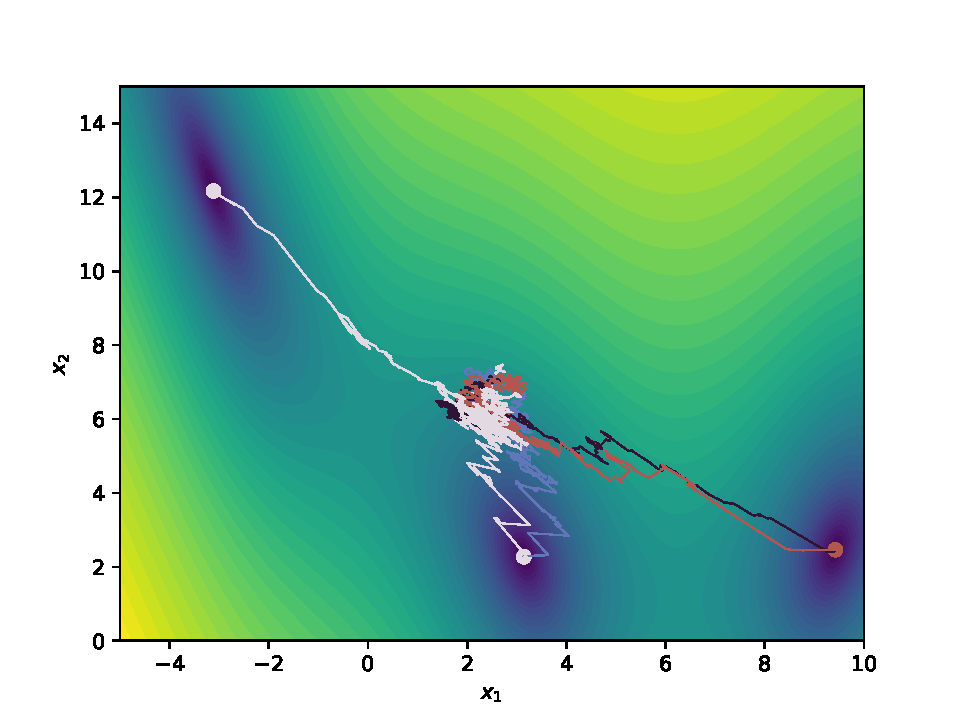
\includegraphics[scale=0.42]{figures/fig51-branin.pdf}
    \label{fig:5.1.1}
\end{figure}

\begin{figure}
    \centering
    \caption{Average SA trajectories for GP}
    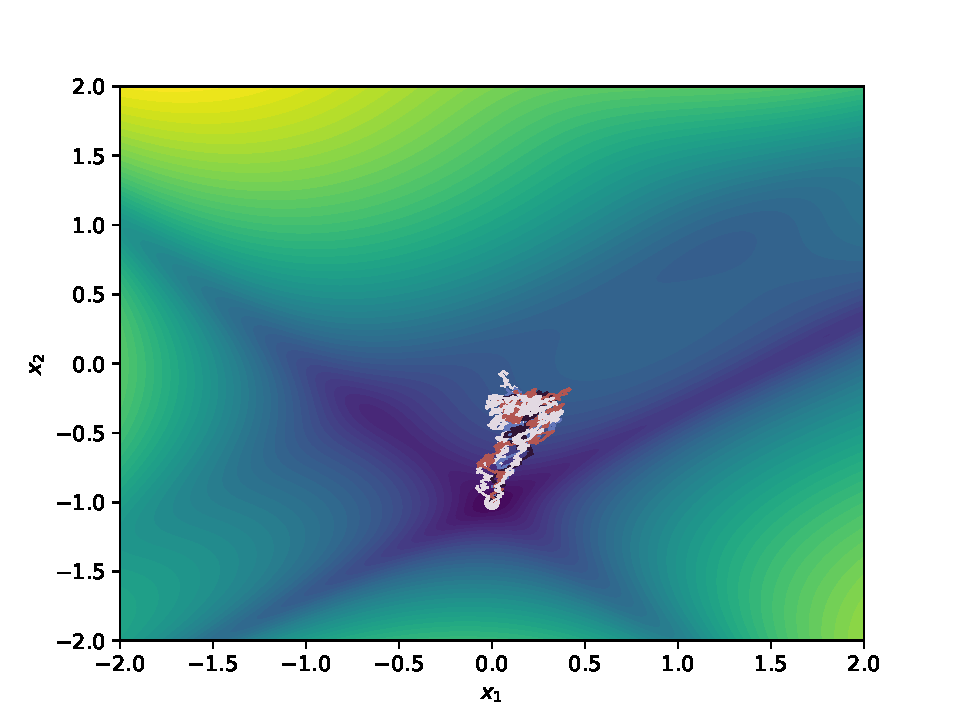
\includegraphics[scale=0.42]{figures/fig51-goldstein_price.pdf}
    \label{fig:5.1.2}
\end{figure}

\begin{table}
    \center
    \caption{Average number of runs required to solve problems}
    \label{table:run_numbers}
    \footnotesize
    \setstretch{1.5}
    \begin{tabular}{cc|cccc}
        & Problem & Avg. num runs & Solutions found & $\# f$ evals & $\# \nabla f$ evals \\
        \hline
1 & RB & 1.0 & 1 & 614.58 & 210.68 \\
1 & GP & 1.6 & 1 & 1072.38 & 385.96 \\
3 & BR & 5.18 & 3 & 3012.68 & 1041.06 \\
1 & H3 & 1.12 & 1 & 575.08 & 211.06 \\
1 & H6 & 1.58 & 1 & 737.7 & 284.1 \\
    \end{tabular}

\end{table}
    
\Cref{table:run_numbers} shows the average required number of runs for the benchmark problems RB, GP, BR, H3, and H6. Simulated Annealing is run
repeatedly until all known global minima are found for the problem. A solution $\hat{\vect{x}}_i$ is considered the same
if $|\hat{\vect{x}}_i - \vect{x}^\star_j|_2 \leq \tau = 10^{-4}$.
This process is repeated $M=50$ times
and the average number of runs, average function and Jacobian values are reported. In all cases, every global minimum
was found. The results show that test problems BR and H6 require a greater average number of required runs per global minima. 

The following
Simulated Annealing parameters were used: $l_0=20, \delta=1.1, \epsilon_s=1e-4, \chi=0.9,
\gamma=10^{-2}$, and $t=0.5$.


\begin{table}
    \center
    \caption{Global and local minima found by Simulated Annealing}
    \label{table:minima}
    \footnotesize
    \setstretch{1.5}
    \begin{tabular}{rc|lr}
        Prob & Type & $\vect{x}^\star_i$ & $f(\vect{x}^\star_i)$ \\
        \hline
RB & g & ( 1.0, 1.0 ) & 0.0 \\
\hline
GP & g & ( -0.0, -1.0 ) & 3.0 \\
& l &( -0.6, -0.4 ) & 30.0 \\
& & ( 1.8, 0.2 ) & 84.0 \\
\hline
BR & g & ( -3.14159, 12.275 ) & 0.39789 \\
& & ( 3.14159, 2.275 ) & 0.39789 \\
& & ( 9.42478, 2.475 ) & 0.39789 \\
\hline
H3 & g & ( 0.11461, 0.55565, 0.85255 ) & -3.86278 \\
& l &( 0.10934, 0.86052, 0.56412 ) & -3.08976 \\
\hline
H6 & g & ( 0.20169, 0.15001, 0.47687, 0.27533, 0.31165, 0.6573 ) & -3.32237 \\
& l &( 0.40465, 0.88244, 0.8461, 0.57399, 0.13893, 0.0385 ) & -3.20316 \\
\end{tabular}
\end{table}

\begin{figure}
    \center
    \caption{Markov chain trajectories for BR}
    \label{fig:markov-traj}
    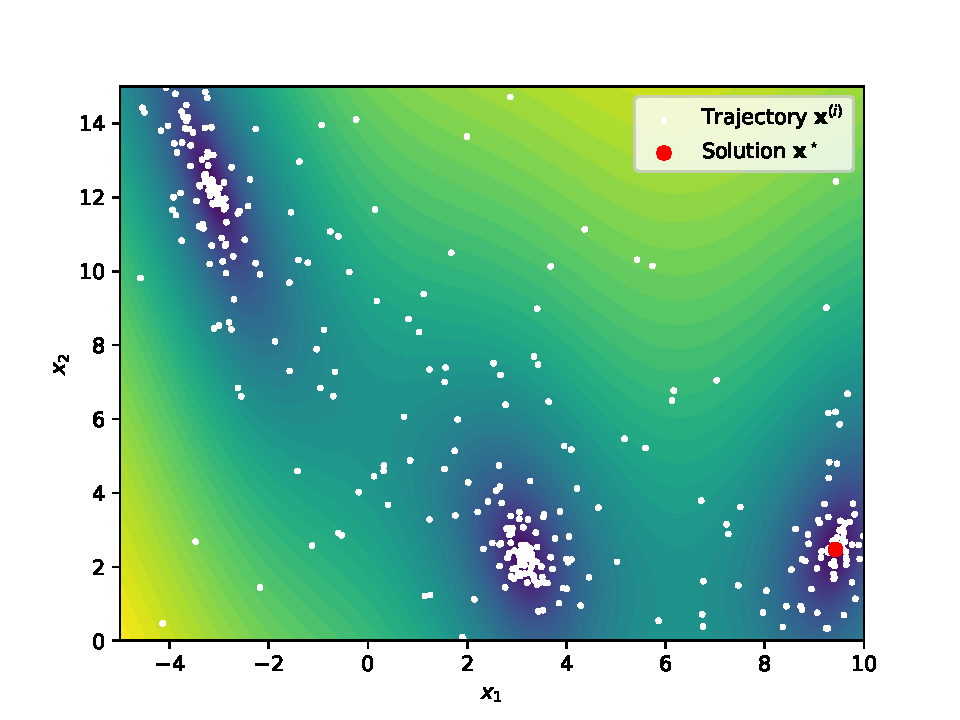
\includegraphics[scale=0.55]{figures/fig-traj.pdf}
    \vspace{10pt}
    \footnotesize
    \setstretch{1.2}
    \flushleft
    \textbf{\Cref{fig:markov-traj}} shows the effective sampling of the test function BR by the Simulated
    Annealing method. White points denote states visisted by the Markov chains. Red denotes the solution
    that this run converged to. Observe how SA oversamples points near the bottoms of the regions of attraction
    of each global minimum.
\end{figure}

\section{Numerical Comparisons}
\label{sec:experiments}

\subsection{MS (Multi-start)}
\label{compare:ms}

Multi-start techniques form a family of heuristic global optimization algorithms. These techniques work in a two-phase
process. In the first global phase, starting points are sampled in the feasible region or domain $\mathcal{S}$ of the
objective function. The most naive implementation of the global phase is to simply perform a uniform sampling of $\mathcal{S}$.
Some members of this family of algorithms utilize sophisticated heuristics to generate starting points such as the
Scatter Search technique.

The local phase of multi-start algorithms use the starting points from the global phase to perform a local optimization
using one of the many algorithms for local optimization. Multi-start algorithms alternate between the global and local
phases until a solution is found \cite{Ugray2007ScatterSA}.

The hardest part of divising an efficient Multi-start method is the selection of an appropriate stopping rule.
Variations in the literature range from several addhoc holes to Bayesian stoppic rules. For the sake of comparison
we utilize a double-box stopping rule [cite box-cstr here].

Let $m(\mathcal{S})$ be the Lebesque measure of the search region $\mathcal{S}$. Since the local search method is
deterministic, in the limit of $n\rightarrow \infty$ runs of the local search method, the algorithm will converge
to $w$ unique local minima. Each local minimum $\vect{x}_i^\star \in\mathcal{S}$ has an associated region of
attraction $A_i$ defined as

$$
A_i := \left\lbrace \vect{x} : \vect{x}\in\mathcal{S}, \texttt{LS}(\vect{x}) = \vect{x}_i^\star \right\rbrace.
$$

Since $\mathcal{S}$ contains $w$ local minima, and the $A_i\cap A_j=\emptyset$, $A_i$ partitions $\mathcal{S}$ i.e.,

$$
\bigcup_{i=1}^w A_i = \mathcal{S}.
$$

Furthermore, if $m(A_i)$ denotes the Lebesque measure of $A_i$, then

$$
m(\mathcal{S}) = \sum_{i=1}^w m(A_i).
$$

If some initial point $\vect{x}_0 \sim \text{Uniform}(\mathcal{S})$, then the probability of $\vect{x}_0$ begin contained
in $A_i$ is simply

$$
P(\vect{x}_0 \in A_i) = \frac{m(A_i)}{m(\mathcal{S})}.
$$

The double-box stopping rule is based on the idea that we want to ensure that all $A_i$ are sampled in $\mathcal{S}$, but
additional sampling results in uncessary computation. Define $C$ has a relative measure of the coverage after the discovery
of $w$ local minima, as

\begin{equation}\label{eq:coverage}
C = \sum_{i=1}^w \frac{m(\mathcal{A}_i)}{m(\mathcal{S})}.
\end{equation}

A sensible heuristic is to stop when $C\longrightarrow 1$. The quantity inside the summation of \cref{eq:coverage} is
not calculatable in practice, but as $w\rightarrow \infty$, we approximate it with

\begin{equation}\label{eq:cov_approx}
C \approx \sum_{i=1}^w \frac{L_i}{L},
\end{equation}

where $L_i$ is the number of starting points of the LS which converged to the local minimizer $\vect{x}_i$, and
$L$ is the total of initial points so far. The quantity in \cref{eq:cov_approx} is equal to 1 by definition, so another
means must be determined. Construct a region $\mathcal{S}_2$ such that $\mathcal{S}\subset \mathcal{S}_2$ and 
$m(\mathcal{S}_2) = 2\cdot m(\mathcal{S})$. For each iteration, we sample from $\mathcal{S}_2$ until we have a point in
$\mathcal{S}$, in other words points in $A_0 = \mathcal{S}_2 \setminus \mathcal{S}$ are discared. Also let
$L_0$ denote the number of sampled points in $A_0$. The total count of sampled points is now given by

$$
L = L_0 + \sum_{i=1}^w L_i,
$$

and the relative coverage $C$ is now

$$
C = \frac{1}{m(\mathcal{S})} \sum_{i=1}^w m(A_i) = 2\sum_{i=1}^w \frac{m(A_i)}{m(\mathcal{S}_2)}
$$

and finally we can approximate relative coverage with

$$
C \approx \frac{2}{L}\sum_{i=1}^w L_i
$$

After $n$ iterations, let $M_n$ denote the number of points in $\mathcal{S}_2$, and $n$ are in $\mathcal{S}$. Then define
$\delta_n := n / M_k$ which has an expectation which in the limit of large $n$

$$
\left\langle \delta \right\rangle_n = \frac{1}{n}\sum_{i=1}^n \delta_i \longrightarrow
\frac{m(\mathcal{S})}{m(\mathcal{S}_2)} = \frac{1}{2}
$$

The variance is $\sigma_n^2(\delta) = \left\langle \delta^2\right\rangle_n - \left\langle\delta\right\rangle^2_n$ which
$\longrightarrow 0$ as $n\longrightarrow \infty$. Finally, the double-box rule is

\subsubsection*{Double-box stopping rule:}

\hfill\\

\textbf{(1)} Continue iterating if new minima are found. \textbf{(2)} If no new minima are found, let $\sigma_\text{last}(\delta)$ be the s.t.d. at the last iteration
at which a minimum was found. Contnue iterating while

\begin{equation}\label{eq:double-box-rule}
    \sigma^2(\delta) < \rho \sigma^2_{\text{last}}(\delta)
\end{equation}

where $\rho \in (0,1)$ is a paramter that performs exhaustive search when $\rho$ is close to 0 and emphasises less iterations
when $\rho$ is close to 1.

\subsubsection*{Constructing $\mathcal{S}_2$ from $\mathcal{S}$:}

\hfill\\

In order to apply the double-box stopping rule, we need to construct the box region $\mathcal{S}_2$ such that
$m(\mathcal{S}_2) = 2\cdot m(\mathcal{S})$. Suppose $\mathcal{S}\in\Real^n$, then we can scale the bounds of $\mathcal{S}
= [l_1, u_1] \times \cdots [l_n, u_n]$ 
by $2^{1/n}$, i.e.,

$$
l_i^{(2)} = l_i - \frac{1}{2}\left( 2^{1/n} - 1\right)\left( u_i - l_i \right)\text{ for } i = 1,\ldots n
$$
$$
u_i^{(2)} = u_i + \frac{1}{2}\left( 2^{1/n} - 1\right)\left( u_i - l_i \right)\text{ for } i = 1,\ldots n
$$

%\begin{algorithm}
%\setstretch{1.4}
%\caption{Multi-start with double-box stopping rule}\label{algo:multistart}
%\vspace{8pt}
%\nosemic
%\SetAlgoLined
%\KwIn{$f:\mathcal{S} \longrightarrow \Real, \nabla f, \mathcal{S}, N, \epsilon_s, \tau, \gamma$}

%$f^\star \longleftarrow \infty$\;

%\;

%\For{$n\in \left\lbrace 1,\ldots, N\right\rbrace$}{
%$\vect{x}_0 \longleftarrow \mathrm{Uniform}\left(\mathcal{S}\right)$ \Comment*{random sample init. point}

%$x_l = \texttt{steepest\_descent}(f, \nabla f, \vect{x}_0, \tau)$ \;

%\If{$f(\vect{x}_l) \leq f^\star$}{
%    $f^\star \longleftarrow f(\vect{x}_l)$ \;
%    
%    $\vect{x}^\star \longleftarrow \vect{x}_l$ \;
%}

%\uIf{$n=0$}{
%    $f^\star_s \longleftarrow C$ \Comment*{$0< C \in\Real$ to prevent 0}
%    $f^\star_s^{(0)} \longleftarrow f_s^\star$ \;
%} \uElse{
%    $f^\star_s^{(0)} \longleftarrow f^\star_s$ \;
%    $f^\star_s = \gamma f^\star + (1-\gamma)f^\star_s^{(0)}$
%    \;
%    \Comment{Stop when smoothed improvement reaches 0}
%    $\Delta_s = f^\star_s^{(0)} - f^\star_s$ \;
%    
%    \Comment{Check stop condition}
%    \If{ $\Delta_s \leq \epsilon_s$}{
%        \KwOut{Solution found $\vect{x}^\star$}
%    }
%}

%\;
%\KwOut{Failed to find solution in $N$ iterations, $\vect{x}^\star$}\;
%}
%\end{algorithm}

\subsection{DE (Differential Evolution)}
\label{compare:de}

Differential Evolution is global, gradient-free stochastic optimization algorithm. This population-based method mutates
each solution candidate by mixing the solution with other members of the  population \cite{storn}.
\emph{scipy.optim.differential\_evolution} is used as comparison.

\subsection{BH (Basin Hopping)}
\label{compare:bh}

Basin-hopping is another two-phase global optimization algorithm inspired by energy minimization of clusters of atoms \cite{wales}.
\emph{scipy.optimize.basinhopping} is used for comparison.

\subsection{Evaluation metrics}

\subsubsection{Solution diversity}

Given that $mathcal{S}$ is partitioned by regions of attraction $A_i$ around each local miminum, one way to measure the
efficiency of a global optimization method is to measure the frequency with which the method converges to each global
minimum. A more efficient method will converge to each global minimum with more uniform probability, implying that
less total iterations are needed to find all the global minima.

Suppose that $f :\mathcal{S}\longrightarrow \Real$ has exactly $w$ global minima. After a large number $M$ of runs,
the method has converged to a global minimum $\vect{x}^\star_i$ $w_i$ times. We can define a \emph{solution diversity score} as

\begin{equation}\label{eq:diversity}
    \xi_M = \sum_{i=1}^w \left| \frac{w_i}{M} - \frac{1}{w}\right|.
\end{equation}

Generally, the regions of attraction $A_i$ for all local and global minima could have different Lebesque measures, so a technique
that uses global uniform sampling would oversample some solutions and undersample others.

An ideal technique would converge to solution $\vect{x}_i$ on $M/w$ occasions after $M$ runs. \Cref{eq:diversity} is
minimized by such a technique yielding uniform convergence to all minima. A lower $\xi_M$ indicates a more efficient algorithm,
whereas if some $\vect{x}_i^\star$ are over represented (and some are under represented), $\xi_M$ would be higher, and thus
indicate an inefficient algorithm.

\subsubsection{Number of evaluations of $f$ and $\nabla f$:}

The number of evalaluations of $f$ and $\nabla f$ is another obvious indication of the computational efficiency of a given
optimization method. Our implementation, and methods to which we compare Simulated Annealing facilate the counting of
these function evaluations in all sub procedures of a given method.

\section{Conclusions}
\label{sec:conclusions}

The work of Dekkers and Aarts have placed Simulated Annealing on a firm rigorous framework that enables further
work and understanding of stochastic global optimization methods.

\subsection{A robust and efficient method}

Our empirical results, achieved with a non-optimized, and rather
crude implementation, show that Simulated Annealing is both a robust and efficient method. Simulated Annealing has
outperformed the chosen global optimization methods provided by

\noindent\texttt{scipy.optimize}, in respect to our multiple
global minima test.

\subsection{Further work}

Simulated Annealing, Multi-start, and the various other methods provided by \texttt{scipy.optimize} were used with
default parameters. Further exploration and analysis should be done to determine optimal parameters for all methods 
to get a more fair comparison between the different methods.

Regrettably, our small selection of test problems had a only a small number of global and local minima. It would be
insightful to explore test problems that have large numbers of minima. It is uncertain if our results would hold
in such a regime.

Lastly, another interesting avenue of exploration would be to develop different methods of point generation for the
Markov chains. Does there exist a way to sample points directly from a probability distribution using function information?
This would avoid the costly and wasteful discarding or a large number of points.



%%
%% The acknowledgments section is defined using the "acks" environment
%% (and NOT an unnumbered section). This ensures the proper
%% identification of the section in the article metadata, and the
%% consistent spelling of the heading.
% \begin{acks}
% To Robert, for the bagels and explaining CMYK and color spaces.
% \end{acks}

%%
%% The next two lines define the bibliography style to be used, and
%% the bibliography file.
\bibliographystyle{ACM-Reference-Format}
\bibliography{bibliography}

\clearpage
%\addbibresource{bibliography.bib}
%\printbibliography


%%
%% If your work has an appendix, this is the place to put it.
\appendix
\section{Benchmark functions used}
\label{apendix:a}

\subsection{RB (Rosenbrock)}

The Rosenbrock function is a widely used non-convex test function with a one global minimum inside of a long, narrow valley.
It is defined as

$$
f\left(x_1, x_2\right):=\left(a-x\right)^2 + b\left(x_2-x_1^2\right)^2
$$

The global minimum is at $\vect{x}^\star=\begin{pmatrix} a & a^2\end{pmatrix}^T$. The typical values are $a=1$ and $b=100$ \cite{rosenbrock}.

\subsection{GP (Goldstein-Price)}

The Goldstein-Price\cite{dekkers} test function in $\Real^2$ is given by

$$
f(x_1,x_2) = \left[ 1 + \left( x_1 + x_2 +1\right)^2
\left( 19-14x_1 + 3x_1^2 - 14x_2 + 6x_1x_2 + 3x_2^2\right)\right]
$$

$$
\times \left[ 30 + \left(2x_1-3x_2\right)^2\left(18-32x_1+12x_2+48x_2-36x_1x_2+27x_2^2\right)\right]
$$

$\mathcal{S} = \left\lbrace \vect{x} : -2 \leq x_i \leq 2, i=1,2\right\rbrace$. It has a global minimum at
$\vect{x}^\star = \begin{pmatrix} 0 & -1\end{pmatrix}^T$.

\subsection{H3 and H6 (Hartmann's family)}
$$
f(\vect{x}) = -\sum_{i=1}^m c_i \exp\left( -\sum_{j=1}^n a_{ij}\left(x_i - p_{ij}\right)^2\right)
$$

where for H3 in $\vect{x}\in\Real^4$, with $m=4$ and $n=3$ is given by

$$
A=[a_{ij}] = \begin{bmatrix}
3 & 10 & 30\\
0.1 & 10 & 35 \\
3 & 10 & 30 \\
0.1 & 10 & 35
\end{bmatrix},
\quad
\vect{c} = \begin{bmatrix} 1 \\ 1.2 \\ 3 \\ 3.2 \end{bmatrix},
$$

$$
P=[p_{ij}] = \begin{bmatrix}
0.3689 & 0.1170 & 0.2673 \\
0.4699 & 0.4387 & 0.7470 \\
0.1091 & 0.8732 & 0.5547 \\
0.038150 & 0.5743 & 0.8828 \\
\end{bmatrix}
$$

where for H6 in $\vect{x}\in\Real^4$, with $m=4$ and $n=6$ is given by

$$
A=[a_{ij}] = \begin{bmatrix}
10 & 3 & 17 & 3.5 & 1.7 & 8\\
0.05 & 10 & 17 & 0.1 & 8 & 14  \\
3 & 3.5 & 1.7 & 10 & 17 & 8 \\
17 & 8 & 0.05 & 10 & 0.1 & 14 
\end{bmatrix},
\quad
\vect{c} = \begin{bmatrix} 1 \\ 1.2 \\ 3 \\ 3.2 \end{bmatrix},
$$

$$
P=[p_{ij}] = \begin{bmatrix}
0.1312 & 0.1696 & 0.5569 & 0.0124 & 0.8283 & 0.5886 \\
0.2329 & 0.4135 & 0.8307 & 0.3736 & 0.1004 & 0.9991 \\
0.2348 & 0.1451 & 0.3522 & 0.2883 & 0.3047 & 0.6650\\
0.4047 & 0.8828 & 0.8732 & 0.5743 & 0.1091 & 0.0381 \\
\end{bmatrix}
$$

\subsection{S5, S7 and S10 (Shekel's Family)}
The Shekel's family of functions, S5, S7, and S10 \cite{dekkers}, is given as:
$$f(x) = -\sum_{i=1}^m ((x-a_i)^T(x-a_i)+c_i)^{-1}$$
which has a dimension of $n=4$, and $m=5$, $m=7$, and $m=10$ for the S5, S7, and S10 respectively. Let $x = (x_1, x_2, ..., x_n)^T$, and $a_i = (a_{i1}, a_{i2}, ..., a_{in})^T$. \vspace{5pt}

Thus for S5:
$$
A=[a_{ij}] = \begin{bmatrix}
4 & 4 & 4 & 4 \\
1 & 1 & 1 & 1 \\
8 & 8 & 8 & 8 \\
6 & 6 & 6 & 6 \\
3 & 7 & 3 & 7 \\
\end{bmatrix},
\quad
\vect{c} = \begin{bmatrix} 0.1 \\ 0.2 \\ 0.2 \\ 0.2 \\ 0.4 \\ 0.4 \end{bmatrix},
$$

Then for S7:
$$
A=[a_{ij}] = \begin{bmatrix}
4 & 4 & 4 & 4 \\
1 & 1 & 1 & 1 \\
8 & 8 & 8 & 8 \\
6 & 6 & 6 & 6 \\
3 & 7 & 3 & 7 \\
2 & 9 & 2 & 9 \\
5 & 5 & 3 & 3 \\
\end{bmatrix},
\quad
\vect{c} = \begin{bmatrix} 0.1 \\ 0.2 \\ 0.2 \\ 0.2 \\ 0.4 \\ 0.4 \\ 0.6 \\ 0.3 \end{bmatrix},
$$

Then for S10:
$$
A=[a_{ij}] = \begin{bmatrix}
4 & 4 & 4 & 4 \\
1 & 1 & 1 & 1 \\
8 & 8 & 8 & 8 \\
6 & 6 & 6 & 6 \\
3 & 7 & 3 & 7 \\
2 & 9 & 2 & 9 \\
5 & 5 & 3 & 3 \\
8 & 1 & 8 & 1 \\
6 & 2 & 6 & 2 \\
7 & 3.6 & 7 & 3.6
\end{bmatrix},
\quad
\vect{c} = \begin{bmatrix} 0.1 \\ 0.2 \\ 0.2 \\ 0.2 \\ 0.4 \\ 0.4 \\ 0.6 \\ 0.3 \\ 0.7 \\ 0.5 \\ 0.5 \end{bmatrix},
$$

\end{document}
\endinput
%%
